\section{Methods}
\label{sxn:methods}


Let us write the Energy Landscape (or optimization function, parameterized by $\mathbf{W}_{l}$s and $\mathbf{b}_{l}$s) for a typical DNN with $L$ layers, with activation functions $h_{l}(\cdot)$, and with $N\times M$ weight matrices $\mathbf{W}_{l}$ and biases $\mathbf{b}_{l}$, as:
\begin{equation}
E_{DNN}=h_{L}(\mathbf{W}_{L}\times h_{L-1}(\mathbf{W}_{L-1}\times h_{L-2}(\cdots)+\mathbf{b}_{L-1})+\mathbf{b}_{L})  .
\label{eqn:dnn_energy}
\end{equation}
We assume we are given several pretrained Deep Neural Networks (DNNs), e.g., as part of an architecture series.
The models have been trained on (unspecified and unavailable) labeled data $\{d_{i},y_{i}\}\in\mathcal{D}$, using Backprop, by minimizing some (also unspecified and unavailable) loss function $\mathcal{L}()$. 
We expect that most well-trained, production-quality models will employ one or more forms of on regularization, such as Batch Normalization, Dropout, etc., and many will also contain additional structure such as Skip Connections, etc. 
Here, we will ignore these details, and will focus only on the weight matrices. 


\paragraph{DNN Quality Metrics.}

Each DNN layer contains one or more layer 2D weight matrices $\mathbf{W}_{L}$, and/or 2D feature maps $\mathbf{W}_{i,L}$ extracted from 2D Convolutional layers. 
(For notational convenience, we may drop the $i$ and/or $i,l$ subscripts below.) 
%
\michael{
XXX.  PROBABLY WE DO NOT WANT THE FOLLOWING.  INSTEAD, JUST PRESENT METRICS AND POINT TO PREVIOUS PAPERS FOR JUSTIFICATION.  E.G., WE DONT WANT TO JUSTIFY THE IMPLICIT STATISTICAL INDEPENDENCE ASSUMPTION HERE.  IF OKAY, JUST DELETE THIS RED BLOCK.
We assume the layer weight matrices are statistically independent, allowing us to estimate the Complexity $\mathcal{C}$, or test accuracy, with a standard Product Norm, which resembles a data dependent VC complexity
\begin{equation}
\mathcal{C}\sim\Vert\mathbf{W}_{1}\Vert\times\Vert\mathbf{W}_{2}\Vert\cdots\Vert\mathbf{W}_{L}\Vert ,
\end{equation}
where $\mathbf{W}$ is an $(N\times M)$ weight matrix, with $N\ge M$, and 
 $\Vert\mathbf{W}\Vert$ is a matrix norm.   We will actually compute the log Complexity, which takes the form 
of an Average Log Norm:
\begin{eqnarray*}
\log\mathcal{C} &\sim& \log\Vert\mathbf{W}_{1}\Vert+\log\Vert\mathbf{W}_{2}\Vert\cdots\log\Vert\mathbf{W}_{L}\Vert
\end{eqnarray*}
}
%
We have examined a large number of possible quality metrics.
The best performing metrics (recall that we can only consider metrics that do not use training/test data) depend on the norm and/or spectral properties of weight matrices, $\mathbf{W}$.%
\footnote{We do not use intra-layer information from the models in our quality metrics, but as we will describe our metrics can be used to learn about }
We consider the following metrics.
\begin{itemize}
\item 
Frobenius Norm: $\Vert\mathbf{W}\Vert^{2}_{F}=\Vert\mathbf{W}\Vert^{2}_{2}=\sum_{i,j}w^{2}_{i,j} = \sum_{i=1}^{M} \lambda_{i}^{2}$
\michael{Do we use norm or log norm, here and with other norms.  Worth being very explicit and very consistent.}
\item 
Spectral Norm: $\Vert\mathbf{W}\Vert_{\infty}=\lambda_{max}$
\michael{We should probably call the spectral norm $\Vert\mathbf{W}\Vert_{2}$, or change Frob norm notation and have an explicit remork.  Let's decide.}
\item 
Weighted Alpha Metric: $\hat{\alpha}=\alpha\log\lambda_{max}$
\item 
$\alpha$-Norm (or $\alpha$-Shatten Norm): $\Vert\mathbf{X}\Vert^{\alpha}_{\alpha}=\sum_{i=1}^{M}\lambda_{i}^{\alpha}$,
\michael{Be clear about how we average this across layers.}
\end{itemize}
The first two metrics are well-known in ML.
The last two deserve special mention.
For all these metrics, $\lambda_{i}$ is the $i^{th}$ eigenvalue of the \emph{Empirical Correlation Matrix},
$ %% $$
\mathbf{X}=\mathbf{W}^{T}\mathbf{W} ,
$ %% $$
and so $\lambda_{max}$ is the maximum eigenvalue of $\mathbf{X}$. 
(These eigenvalues are the squares of the singular values $\sigma_{i}$ of $\mathbf{W}$, i.e., $\lambda_{i}=\sigma^{2}_{i}$.)
For the last two metrics, the exponent $\alpha$ is the power law exponent that arises in the recently-developed \emph{Theory of Heavy Tailed Self Regularization (HT-SR)}~\cite{MM18_TR, MM19_HTSR_ICML, MM20_SDM}.
Operationally, $\alpha$ is determined by using the publicly-available \emph{WeightWatcher} tool (\cite{weightwatcher_package}) to fit the Empirical Spectral Density (ESD) of $\mathbf{X}$, i.e., a histogram of the eigenvalues, call it $\rho(\lambda)$, to a truncated power law
\begin{equation}
\rho(\lambda)\sim\lambda^{\alpha},\;\;\lambda\le\lambda_{max}  .
\end{equation}
\michael{We need to be clear that this is a truncated power law fit and that $\lambda_{max}$ comes from that and not the largest empirical eigenvalue.}
The Weighted Alpha Metric was introduced previously~\cite{MM20_SDM}, where (on a much smaller set of data than we consider here) it was shown to correlate well with the trends in reported test accuracies of pretrained DNNs.
Based on this, here we introduce and evaluate the $\alpha$-Norm metric.
One would expect $\hat{\alpha}$ to approximate the log $\alpha$-Norm very well for $\alpha < 2$ and reasoably well for $\alpha\in[2,5]$~\cite{MM20_unpub_work}.

\michael{Need to say that such large $\alpha$ values don't mean much.}

\michael{Need to highlight difference between $\alpha$ and $\hat{\alpha}$.}


\paragraph{Spectral Analysis of Convolutional 2D Layers.}

There is some ambiguity in performing spectral analysis on Convolutional 2D (Conv2D) layers.  
A Conv2D layer can be represented as a 4-index tensor of dimension $(w,h,in\_ch,out\_ch)$, specified by an $(w\times h)$ filter (or kernel) and $in\_ch$ / $out\_ch$ input / output channels, respectively (usually $in\_ch\le out\_ch$). 
Typically, $w=h=k$,  giving $(k\times k)$ tensor slices, or \emph{pre-Activation Maps} $\mathbf{W}_{i,L}$ of dimension $(in\_ch\times out\_ch)$ each. 
%
There are at least three different approaches that have been advocated for applying the Singular Values Decomposition (SVD) to an Conv2D layer:
run an SVD on each of the pre-Activation Maps $\mathbf{W}_{i,L}$, yielding $(k\times k)$ sets of $M$ singular values; 
stack the feature maps into a single rectangular matrix of, say, dimension $((k\times k\times out\_ch)\times in\_ch)$, yielding $in\_ch$ singular values;
compute the 2D Fourier Transform (FFT) for each of the $(in\_ch, out\_ch)$ pairs, and run SVD on the resulting Fourier coeffients~\cite{Long2019}, leading to $\sim(k\times in\_ch\times out\_ch)$ non-zero singular values.
Each method has tradeoffs.  
In principle, the third method is mathematically sound, but it is computationally expensive. 
For our analysis, because we are performing tens of thousands of calculations, we select the first method, which is numerically the fastest and is easiest to reproduce.%
\footnote{We provide a Google Colab notebook where all results can be reproduced, with the option to redo the calculations with the third option for the SVD of the Conv2D.}


\paragraph{XXX.}
XXX.  THIS VERIFICATION IS NOT ABOUT CONV LAYERS, IT IS ABOUT PL MORE GENERALLY, CORRECT?  WE SHOULD CLARIFY AND SQUISH.
To verify that our approach is meaningful, we need to confirm that the ESD is neither due to a random matrix, nor due to unsually large matrix elements, but, in fact, captures correlations learned from the data. 
We examine typical layer for the pretained AlexNet model (distributed with pyTorch). 
Figure~\ref{fig:alexnet1} displays the ESD for the first slice (or matrix $\mathbf{W}$) of the third Conv2D layer, extracted from a 4-index Tensor of shape $(384, 192, 3, 3)$.  The red line displays the best fit to a random matrix, using the Marchenko pastur theory~\cite{MM}.  We can see the random matrix model does not describe the ESD very well. For comparison, Figure \ref{fig:alexnet2} shows the ESD of the same matrix, randomly shuffled; here looks similar to the red line plot of the orginal ESD.  In fact, the empircal ESD is better modeled with a truncated power law distribtion.
\michael{We may want to give a one-sentence summary of this par and fig at the end of the previous par.}

\begin{figure}[H]
   \centering
   \subfigure[Actual ESD]{
     %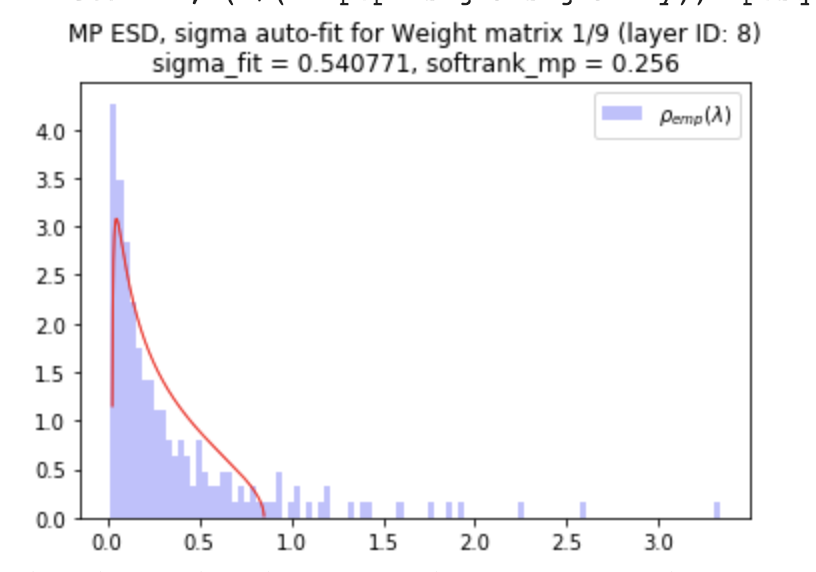
\includegraphics[scale=0.5]{img/alexnet1.png} 
     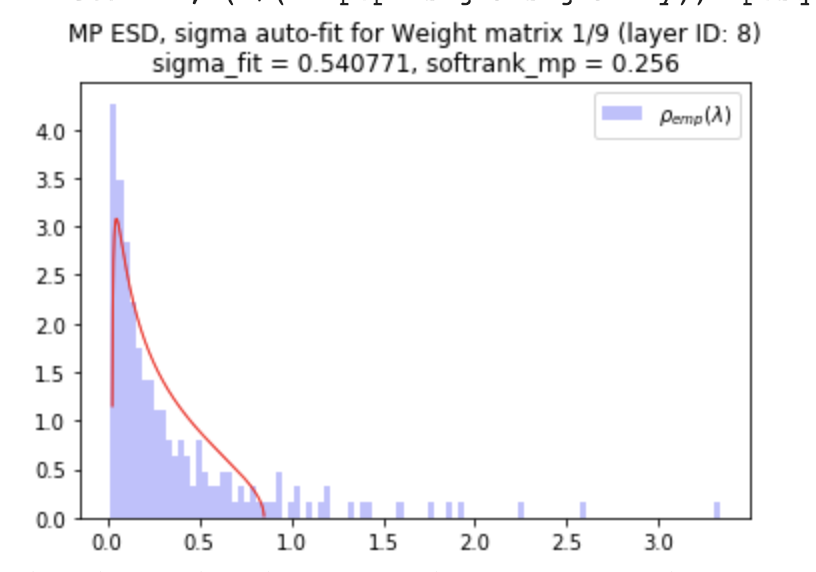
\includegraphics[scale=0.25]{img/alexnet1.png} 
     \label{fig:alexnet1}
   }
   \subfigure[ESD of randomly shuffled matrix]{
      %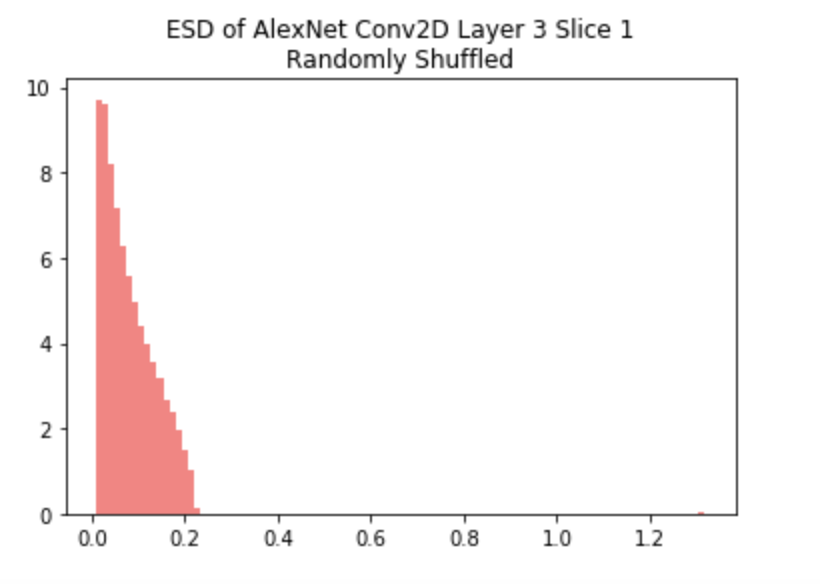
\includegraphics[scale=0.5]{img/alexnet2.png}
      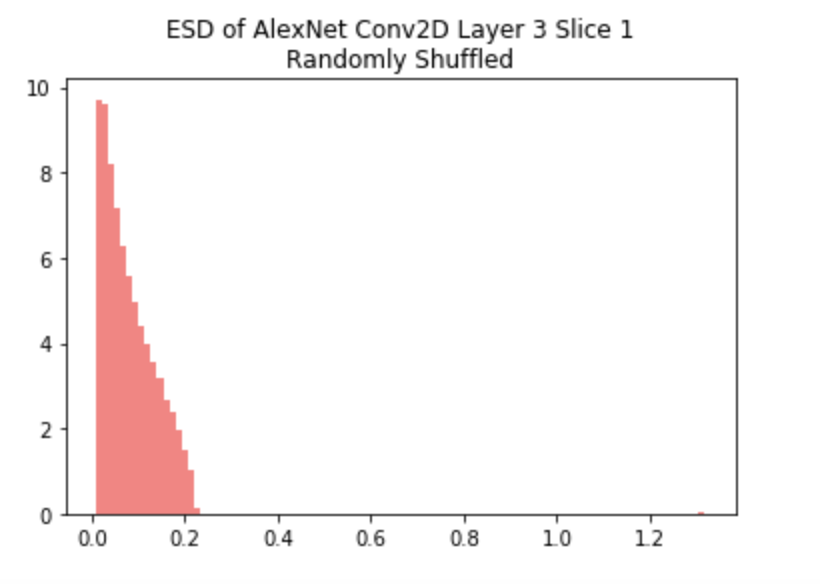
\includegraphics[scale=0.25]{img/alexnet2.png}
      \label{fig:alexnet2}
   }
   \caption{ESD of AlexNet Conv2D pre-Activation map for Layer 3 Slice 1, actual and randomized.
            \michael{Need better figs here.}
           }
   \label{fig:alexnet}
\end{figure}


Although the ESD is \emph{Heavy Tailed}, this does not imply that the orginal matrix $\mathbf{W}$ is itself heavy tailed--only the correlation matrix $\mathbf{X}$ is. 
If $\mathbf{W}$ was, then it would contain 1 or more unusually large matrix elements, and they would dominate the ESD.  
Of course the randomized $\mathbf{W}$ would also be heavy tailed, but its ESD neither resembles the original nor is it heavy tailed. 
So we can rule out $\mathbf{W}$ being heavy tailed.
\michael{These comments seem out of place, since they hold more generally than for the Conv2D layers.}

These plots tell us that the pre-activation maps of the Conv2D contains significant correlations learned from the data.  
By modeling the ESD with a power law distribution $\lambda^{\alpha}$, we can characterize the amount of correlation learned;
the smaller the exponent $\alpha$, the more correlation in the weight matrix. 
\michael{These comments seem out of place, since they hold more generally than for the Conv2D layers.}

\paragraph{Normalization of Empirical Matrices.}  
Normalization is an important, if underappreciated, practical issue.
Importantly, the normalization of weight matrices does \emph{not} affect the Power Law fits because the Heavy Tailed exponent $\alpha$ (as well as other metrics such as the Stable Rank and MP Soft Rank~\cite{MM18_TR,MM19_HTSR_ICML}) is scale-invariant.
Norm-based metrics, however, do depend strongly on the scale of the weight matrix.
Typically, to apply RMT, we would usually define Correlation Matrix with $1/N$ normalization and assume that the variance of $\mathbf{X}$ is either unity or a known constant.% 
\footnote{For formal proofs of Heavy Tailed results, one typically needs a different normalization such as $1/N^{1-\alpha}$.}
Pretrained DNNs are typically initialized with random weight matrices $\mathbf{W}_{0}$, with the variance already normalized to $\sqrt{1/N}$, or some variant of this, e.g., the Glorot/Xavier normalization~\cite{GloRot}, or a $\sqrt{2/Nk^2}$ normalization for Convolutional 2D Layers.
We do not have conrol over the final empirical normalization of these models; and we do \emph{not} normalize (or renormalize) the Empirical Correlation Matrices, i.e., we use them as-is.
The only exception to this is that we do rescale the Conv2D pre-Activation Maps $\mathbf{W}_{i,L}$ by $k/\sqrt{2}$ so that they are on the same scale as the Linear layers.

\michael{MOVE TO LATER: COMMENT ON HOW LOG NORM first and last layers behave, maybe somewhere else.}

\michael{CMOVE TO LATER: OMMENT ON HOW LOG PORM  for GPT includes unusually high alpha, not meaningful other than to show the trend.}

\paragraph{The WeightWatcher Tool.}

We compute the metrics using the WeightWatcher tool (version 0.2.7), and we provide Jupyter notebooks in the github repo for this paper~\cite{repo}, making the results fully reproducible.

\michael{XXX.  FEW SENTENCES ABOUT REPRODUCIBILITY MORE GENERALLY HERE.}


